% - Fórmula con la que funciona el interferometro
% - Expectativa vs mediciones

\documentclass[a4paper, 12pt]{article}
\usepackage[utf8]{inputenc}
\usepackage[left=1cm, right=1cm, top=1cm, bottom=1cm]{geometry}
\usepackage{indentfirst}
\usepackage[spanish]{babel}
\usepackage{fancyhdr}
\usepackage{graphicx}
\usepackage{amsmath}


\pagestyle{fancy}
\fancyhf{}
\renewcommand{\headrulewidth}{0pt}
\renewcommand{\footrulewidth}{0pt}
\fancyfoot[R]{pág. \thepage}
\setlength{\footskip}{20pt}

%opening
\title{\textbf{\textit{El interferómetro}}}
\author{por Marcos Raúl Gatica - Leg. 402006 - Física Electrónica 2R1}
\date{}

\setlength{\parindent}{2em}

\begin{document}

	\thispagestyle{fancy}
	\maketitle
	\thispagestyle{empty}
	\begin{figure}[h!]
		\centering
		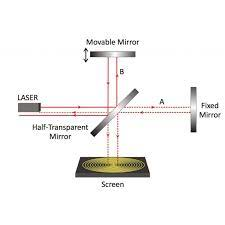
\includegraphics[width=0.8\textwidth]{./imágenes/interferometro2.jpg}
		\caption{Interferómetro de Michelson.}
		\label{fig:interferometro}
	\end{figure}
	
	\newpage
	
	\setcounter{page}{1}
	\tableofcontents

	\newpage
	
	\section{\textbf{Conceptos previos}}
	
	\subsection{La interferencia}
	\indent La interferencia es un fenómeno que ocurre cuando dos o más ondas, de cualquier especie como las electromagnéticas o mecánicas, se traslapan en el espacio. Cuando esto ocurre, la onda total en cualquier punto e instante estará bajo el \textbf{principio de superposición.}
	
	\subsection{El principio de superposición}
	\indent Este principio describe cómo las ondas interactúan cuando se encuentran en el mismo espacio: \textit{"cuando dos o más ondas se interceptan en un mismo punto en el espacio, la amplitud resultante de la onda en ese punto es una suma algebraica de las amplitudes de las ondas individuales"}
	
	\textbf{Ejemplo:} \newline
	\indent Dada la colisión entre dos ondas sinusoidales de la misma frecuencia y magnitud, el punto de colisión genera una onda resultante igual a:
	
	\begin{center}
		${y_1} = A.sen(kx - \omega t)$ \\ 
		${y_2} = A.sen(kx - \omega t)$ \\ \
		
		${y_{RT}} = {y_1} + {y_2}$ \\
		${y_{RT}} = 2A.sen(kx - \omega t)$ \\
	\end{center}
	
	\subsection{Interferencia constructiva y destructiva}
	
	\section{\textbf{El interferómetro}}

	\indent El interferómetro es un dispositivo usado para medir ondas de luz o de sonido mediante el principio de interferencia. Es usado en diversas ramas de la física para detectar pequeñas distancias, movimientos o cambios en una señal.
	
	\indent El dispositivo se usa en varios campos como la astronomía para medir el diámetro de estrellas o la distancia entre cuerpos celestes, y en la medición de ondas gravitacionales (interferómetro láser LIGO).
	
	\section {\textbf{Principio de funcionamiento}}

	\indent El interferómetro se basa en la superposición de ondas, generalmente de la luz. Este fenómeno de interferencia es el que permite detectar variaciones extremadamente pequeñas.
	
	\section{\textbf{El interferómetro de Michelson: estructura típica}}
	
	\indent Es uno de los interferómetros más conocidos, su estructura básica incluye: 
	
	\begin{figure}[h!]
		\centering
		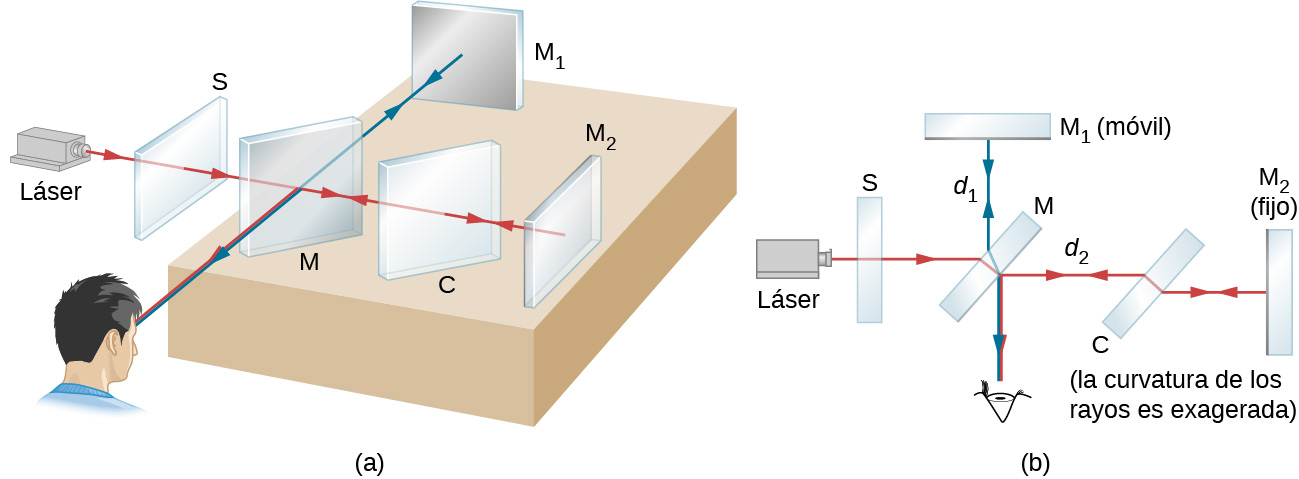
\includegraphics[width=0.75\textwidth]{./imágenes/interferometroDibujoCompleto.jpg}
		\caption{Interferómetro de Michelson - Esquema}
		\label{fig:interferometro2}
	\end{figure}
	
	\begin{enumerate}
		\item \textbf{Fuente de luz:} Se usa una luz coherente, como un láser.
		\item \textbf{Divisor de haz:} Este dispositivo divide el haz de luz en dos partes.
		\item \textbf{Espejos:} Dos espejos colocados en ángulos precisos reflejan los haces divididos.
		\item \textbf{Superposición de los haces:} Los haces de luz vuelven a unirse después de recorrer diferentes caminos, y el patrón de interferencia que se crea se observa en una pantalla o detector.
	\end{enumerate}
	\newpage
	\subsection{Matemática: Fórmula de interferencia de Michelson}
	
	El interferómetro de Michelson crea un patrón de interferencia que depende de la diferencia en la longitud de los caminos recorridos por los dos haces de luz. La fórmula para el número de franjas de interferencia observadas en el patrón es:
	
		\begin{center}
			N = $\frac{2 \Delta L}{\lambda}$ \\
		\end{center}
		
	siendo:
		\begin{itemize}
			\item N: número de franjas de interferencia.
			\item $\Delta L$: diferencia en la longitud de los caminos recorridos por los dos haces de luz.
			\item $\lambda$: longitud de onda de la luz utilizada.
		\end{itemize}
		
	\subsection{Funcionamiento}
		\begin{enumerate}
			\item \textbf{División del haz de luz:} Un haz de luz coherente, como un láser, es dividido en dos haces por un divisor.
			\item \textbf{Reflexión en los espejos:} Los dos haces reflejados viajan por caminos diferentes (espejos y divisor de haz) y luego se recombinan en el divisor de haz.
			\item \textbf{Superposición e interferencia:} Los dos haces se superponen y crean un patrón de interferencia en una pantalla o detector. La diferencia en las distancias recorridas por los haces causa una variación en el patrón de interferencia.
			\item \textbf{Detección de desplazamientos:} Si uno de los espejos se mueve, cambiará la diferencia en las longitudes de los caminos ($\Delta L$), lo que hará variar el número de franjas de interferencia observadas. 
		\end{enumerate}
		
		\textbf{\underline{Aplicación:}} \newline
		\indent Dada una luz cuya longitud de onda sea de 500nm, deseamos medir la diferencia en la longitud del camino de 1micrómetro, usando la Fórmula podemos decir que:
		\begin{center}
			$N = \frac{2 \Delta L}{\lambda}$  \\ \
			\newline
			$N = \frac{2(10^{-6})}{500(10^{-9})}$  \\ \
			\newline
			$N = 4$ \\
		\end{center}
		Esto da a entender que veremos 4 franjas de interferencia moviéndose en respuesta a un cambio de 1 micrómetro en la longitud del camino.
\end{document}
